
% Main tex file for Alex Ledger's thesis

\documentclass[12pt,twoside]{reedthesis}
\usepackage{graphicx,latexsym} 
\usepackage{amssymb,amsthm,amsmath}
\usepackage{longtable,booktabs,setspace} 
\usepackage[hyphens]{url}
\usepackage{rotating}
\usepackage{hhline}
\usepackage{multirow}
\usepackage{adjustbox}
\usepackage{algorithm,algpseudocode}
\usepackage{changepage}
\usepackage{circuitikz}
\usepackage{protocolj}
\usepackage{xspace}

\usepackage{natbib}

\input{macros}

\usepackage{hyperref}
\hypersetup{
    colorlinks=true,
    linkcolor=blue,
    filecolor=magenta,      
    urlcolor=cyan,
}

% Comment out the natbib line above and uncomment the following two lines to use the new 
% biblatex-chicago style, for Chicago A. Also make some changes at the end where the 
% bibliography is included. 
%\usepackage{biblatex-chicago}
%\bibliography{thesis}

\title{Implementing Improvements for Secure Function Evaluation}
\author{Alex Ledger}
\date{May 2016}
\division{Mathematics and Natural Sciences}
\advisor{Adam Groce}
\department{Mathematics}
\setlength{\parskip}{0pt}

\begin{document}

\maketitle
\frontmatter % this stuff will be roman-numbered
\pagestyle{empty} % this removes page numbers from the frontmatter


%!TEX root = thesis.tex


\chapter*{Acknowledgements}
%I would first like to thank my thesis advisor Adam Groce. 
%He has been a great advisor and mentor over the last few years. 
%I would also like to thank my collaborators Alex Malozemoff and Arkady Yerukhimovich
%
%I would like to thank all of my friends; it seems like it's been a lot longer than four runs, but it was a good run. 
%Of all my friends, I would like to especially thank Cat. 
%Cat you have been an amazing companion throughout my time at Reed, and I'm sure at times that I didn't express nearly as much gratitude as I felt. 
%I wouldn't have been able to do Reed with you. 
%
%Finally, I would like to thank my parents and brother.
%You guys mean so much to me; I should probably call you more. 





% The preface is optional
% To remove it, comment it out or delete it.
\chapter*{Preface}
This is an example of a thesis setup to use the reed thesis document class.

\chapter*{List of Notation}

\begin{table}[h]
\centering % You could remove this to move table to the left
\begin{tabular}{ll}
    $W_i$ & Wire i \\
    $W_i^j$ & Wire $i$'s $j$th wire label. $j \in \{0,1\}$ \\
    $W_i^*$ & An unknown wire label of wire $W_i$ \\
    $\sigma_i$ & The semantic value of wire $W_i$ \\
    $\C$ & A circuit \\
    $\GC$ & A garbled circuit \\
    $c$ & A component-circuit \\
    $e_{\C}$ & set of $\C$'s input wires \\
    $d_{\C}$ & set of $\C$'s output wires \\
    $\Delta$ & The delta value for the Free XOR technique \\
    $G_i$ & The $i$th gate \\
    $T_g$  & Garbled table for gate $g$ \\
    $L_{ij}$ & Link label for mapping output wire $W_i$ to input wire $W_j$. \\
    $x$ & Alice's input string \\
    $x_i$ & The $i$th bit of string $x$. \\
    $y$ & Bob's input string \\
    $z$ & he output string \\
    $\gamma \gets 3$ & $\gamma$ is assigned the value $3$ \\
    $\gamma \samples \{0,1\}^n$ & $\gamma$ is sampled uniformly at random from the set $\{0,1\}^n$. \\
\end{tabular}
\end{table}
	
\tableofcontents

\listoftables

\listoffigures

%!TEX root = thesis.tex

\chapter*{Abstract}

Secure computation is a cryptographic method to securely compute a function between two parties while preserving the privacy of the parties' inputs.
Modern secure computation techniques use an offline/online scheme, where parties pre-process and exchange information in an offline phase prior to computing the function in an online phase. 
The offline/online setting has many advantages, namely that the online computation is very fast, but the setting is limiting, as the function that is being computed must be determined ahead of time.

This thesis is part of a larger project studying component-based garbled circuit schemes which aim to improve the offline/online model.
Component-based garbled circuits observe that many real-world functions are composed of many standard components such as arithmetic operations, matrix operations and other common operations.
Component-based garbled circuits exchange many small, generic garbled components in an offline phase. 
Later in the online phase, the parties choose a function they wish to compute, and stitch together the garbled components in order to create the function.

As a part of this larger project, this this contributes two items.
The first is an improvement of component-based garbled circuits called \textit{Single Communication Multiple Connections} (SCMC).
SCMC dramatically reduces the online bandwidth of component-based garbled circuits by observing that there are common patterns when linking garbled components.
This thesis also contributes an implementation, \CompGC, of component-based garbled circuits in the C-programming language. 
We run performance measurements on \CompGC, and we find that component-based garbled circuits offer considerable savings in online time and online bandwidth over other implementations of garbled circuits. 


%\input{dedication}
	
\mainmatter % here the regular arabic numbering starts
\doublespacing
\pagestyle{fancyplain} % turns page numbering back on

%!TEX root = thesis.tex


%The \introduction command is provided as a convenience.
%if you want special chapter formatting, you'll probably want to avoid using it altogether
\chapter*{Introduction}
     \addcontentsline{toc}{chapter}{Introduction}
\chaptermark{Introduction}
\markboth{Introduction}{Introduction}

Secure computation is a cryptographic method that allows two parties who do not trust each other to work together. 
Specifically, the two parties can compute a function $f(x,y)$, where each party keeps their input to the function, $x$ and $y$, private from the opposing party.

The classic example of secure computation is the millionaire problem.
In the millionaire problem, millionaires Alice and Bob wish to determine who is wealthier, but they do not want to disclose their wealth to the opposing party.
Alice and Bob could tell a trusted third party their wealth, and then that trusted third party tells Alice and Bob who is wealthier.
However that method has many disadvantages, one being that they need to trust a third party - what if they can't find a trusted third party?
Secure computation gives Alice and Bob a method to solve their problem without the aid of a third party; they exchange messages between each other and acquire an answer to their question.

Secure computation can be performed for arbitrarily many parties, but this thesis focuses on the special case where two parties are involved; this is called two-party computation (2PC).
The most common method for performing 2PC is \textit{garbled circuits}.
In a garbled circuits protocol, the parties transform their function $f$ into a circuit. 
They then encrypt, or garble their circuit, obscuring the values in the circuit, such that with a bit more information, they recover the answer to their function.

Garbled circuits have been heavily researched and optimized since their creation in the late 1980s.
For most of that period, garbled circuit protocols were too slow and cumbersome for usage in the real world, but as of late, the protocols have achieved speeds comparable to that of loading a webpage. 

In order to further increase the speed of garbled circuits, researchers split the garbled circuit protocol into two phases, an offline phase and an online phase.
In the offline phase, before the two parties determine their inputs to the function, the parties exchange as much information as feasible. 
Then upon determining their inputs to the function, the parties engage in an online phase, where they exchange more information and finish the garbled circuit protocol, recovering the output to their function.
Using an offline/online protocol greatly reduces the latency of the computation - the time that it takes to acquire an answer from the time that the parties determine their inputs.

The offline/online system, while offering a number of benefits, is also limiting in that the function is determined ahead of time in the offline phase.
Say that millionaires Alice and Bob originally agree to find out who is wealthier, so they exchange information for that function ahead of time in the offline phase, but what if at the beginning of the online phase, Alice and Bob change their minds. 
They now wish to simply verify that they are indeed both millionaires, and that the other is not going bankrupt.
Since they exchanged information specific to the ``who is wealthier'' function during the offline phase, they are stuck. 
They cannot pivot and compute the new function without large computational sacrifices.

A new method called \textit{component-based} garbled circuits solves this problem.
In the offline phase, instead of exchanging information corresponding to a single function, Alice and Bob exchange smaller pieces of information that can be stitched together to compute a class of functions.
For example, instead of exchanging a garbled circuit that computes the ``who is wealthier'' function, Alice and Bob exchange a many garbled circuits which are \textit{components} or subparts of the less than function and other similar functions.
Then, during the online phase, Alice and Bob select the function that they wish to compute from the class of available functions, and build their function by \textit{chaining} pre-exchanged components.
With chaining, Alice and Bob have more flexibility. 
They are no longer stuck using their original function - they can securely compute a host of functions at their whim. 

This thesis contributes a new method that improves the efficiency of component-based garbled circuits. 
The original component-based garbled circuits requires that a ciphertext be communicated per wire chained - in other words, the communication scales linearly with the size of data.
Our new method, called Single Communication Multiple Connections (SCMC), requires a single cipher text be communicated per block of data instead of per wire. 
The communication requirement for chaining is now constant in the size of the data object: chaining a $10$ by $10$ matrix has the same bandwidth requirement as chaining a $1,000$ by $1,000$ matrix. 
This allows for extremely fast computation of large statistical operations. 

The major contribution of this thesis is the implementation of component-based garbled circuits and SCMC into a program called \CompGC. 
\CompGC is a full-fledged secure computation system, where parties connect via TCP to agree on a function, exchange inputs, and securely compute the function.
The program is fast, beating the best timings in the literature even for functions that do not benefit the most from SCMC.

This thesis can be read from cover to cover, but it may be useful to skip around.
The first chapter introduces cryptographic primitives, cryptographic knowledge that is needed to understand the more complex cryptographic constructions.
The second chapter discusses what it means for a secure computation protocol to be secure, and introduces garbled circuits, the basic building block of secure computation used in this thesis.
The third chapter presents a variety of improvements to garbled circuits.
The fourth chapter explains component-based garbled circuits, how to chain garbled circuits, and my improvement to chaining, SCMC.
The fifth chapter discusses our implementation of component-based garbled circuits and SCMC, \CompGC, and also gives performance metrics of \CompGC for various functions and settings.









%!TEX root = thesis.tex
\chapter{Cryptographic Primitives}
Secure Compuation is the study of computing functions in a secure fashion. 
SC is split into two cases: cases where there are two parties involved, referred to as two-party computation (2PC), and cases where there are three or more parties, referred to as multiparty computation (MPC).
This thesis will focus primarily on 2PC protocols, but many of the methods are applicable to MPC as well.

2PC protocols are complex cryptographic protocols that rely on a number of cryptographic primitives.
In order to understand 2PC, it is not crucial to understand how the cryptographic primitives work, but it is important to understand their inputs, outputs and security guarantees. 
This first chapter will give an overview of the cryptographic primitives used in 2PC protocols.

\section{Introducing Cryptographic Security} 
The goal of this section is to explain cryptographic security, starting at an intuitive level and moving outward. 
We do not present cryptographic security in a comprehensive fashion; rather, we explain cryptographic security with the goal of explaining 2PC protocols and their security.
For more information on cryptographic security, we encourage the reader to peruse \cite{katzlindelltextbook}. 

We define a few intuitive terms to get started.
A \textit{cryptographic scheme} is a series of instructions designed to perform a specific task. 
An \textit{adversary} is an algorithm that tries to \textit{break} the scheme. 
If an adversary \textit{breaks} a scheme, then the adversary has learned information about inputs to the scheme that they shouldn't. 

The goal of defining security in cryptography is to build a formal definition that matches real world needs and intuitions. 
A good starting place is to consider perfect security. 
A scheme is perfectly secure if no matter what the adversary does, they cannot break the scheme.
Even if the adversary has unlimited computational power, in terms of time and space, an adversary cannot break a perfectly secure scheme. 

However, perfect security is not the most useful way to think of security, because it makes forces schemes to be slow and communication intensive.
We relax the definition of security by requiring that the adversary run in polynomial time. 
This substantially reduces the power of the adversary, and it matches our intuition. 
We are really only concerned with what adversaries can reasonably achieve, as opposed to theoretically possible. 

Because computers have improved drastically over the years, what was previously considered a reasonable adversary is not what is considered a reasonable adversary today. 
Modern computing advances have created easy access to faster computation, meaning that modern adversaries can solve harder problems than they could in previous years. 
As a concrete example, consider an giving an adversary the following problem: find the factors of $N$. 
The average computer today can solve the problem for a larger $N$ than the average computer a decade ago.

Changing computational power makes it important to scale how hard a cryptographic scheme is to break.
To this end, we introduce a \textit{security parameter}, denoted as $\lambda$.
A security parameter is a positive integer that represents how hard a scheme is to break. 
A larger security parameter should mean that the scheme is more difficult to break. 
More specifically, the security parameter is correlates to the input-size of the problem underlying the cryptographic scheme. 
For example, if the underlying problem is factoring large number $N$, then $N = \lambda$. 
As $N$ and $\lambda$ scale up, the factoring problem becomes more difficult and the scheme becomes hard to break. 

Finally, we acknowledge that adversaries have access to some random values, hence we strengthen adversaries to be probabilistic algorithms. 
Probabilistic means that the algorithms have access to a string of uniform random bits, with the implication being that the algorithm is capable of guessing. 

In order to reason about the security of cryptographic schemes, it is useful to think about breaking a scheme in terms of a probability. 
For example, we want to be able to say that the best adversary, that is best probabilistic polynomial-time algorithm, has some probability $p$ of breaking the scheme. 
We note that $p$ is nonzero, since the adversary can always guess and be right with some nonzero probability. 
To achieve a probability based formalism, we introduce a negligible function.
Informally, a negligible function is smaller than the reciprocal of all polynomial functions. 
Formally, a negligible function is:

\begin{definition}
\label{defn:negible}
A function $\mu : \NN \to \RR$ is negligible if for all positive polynomial $p(\cdot)$, there exists positive integer $N_p$ such that for all $x > N_p$, 
\begin{equation}
    |\mu(x)| < \frac{1}{p(x)}.
\end{equation}
\cite{goldreich}
\end{definition}

Examples of negligible functions include $2^{-n}$, $2^{- \sqrt{2}}$ and $n^{- \log n}$. 

To put a negligible function to use, say an adversary is attacking a cryptographic scheme that is equivalent to solving a problem $P$ with input-size $\lambda$ and $2^{\lambda}$ possible answers. 
Moreover, say that $P$ is known to be NP-hard such that there is no polynomial time algorithm to solve $P$. 
Then, the best that the adversary can do is to guess the answer to $P$.
Hence the probability that the adversary that finds the answer the $P$, or breaks the scheme, is 
\begin{align*}
Pr[\text{A correctly answers $P$}] & = {2^{- \lambda}}
\end{align*}
Since $2^{- \lambda}$ is a negligible function, we say that the adversary has a negligible probability of breaking the scheme. 

In summary, we model an adversary as a probabilistic polynomial-time algorithm. 
This limits the computational power of the adversary to what is reasonably computable in reality. 
Moreover, we can scale the security of a scheme or problem by changing $\lambda$, the security parameter. 
A higher security parameter makes the scheme more difficult to break. 

\section{Encryption}

Encryption is the process of obfuscating a message, and then later un-obfuscating the message.
Say Alice has a message that she wants to send to Bob, but somewhere between Alice and Bob sits Eve, who wants to learn about the message.
An encryption scheme enables Alice to send her message to Bob with confidence that Eve cannot learn any information about the message. 

An encryption scheme is composed of three algorithms: $\Enc$, $\EncInv$ and $\Gen$; formally, we say an encryption scheme is a tuple $\Pi = (\Gen, \Enc, \EncInv)$\footnote{We use $\Pi$ here to denote the encryption scheme, because it is a protocol. Protocol starts with a p.}.
$\Enc$ the obfuscating algorithm, $\EncInv$ is the un-obfuscating algorithm and $\Gen$ generates a key. 
The key is extra information that $\Enc$ and $\EncInv$ use to obfuscate and un-obfuscate the message respectively. 
The key, denoted $k$, is a random\footnote{The notion of randomness in cryptography is precisely defined, and in cases where $\lambda$ is large, it is sufficient for $k$ to be pseudorandom. Pseudorandomness is also precisely defined.} string of $\lambda$ bits, that is $k$ is randomly sampled from $\{0,1\}^{\lambda}$  where $\lambda$ is the security parameter of the encryption scheme. 
As per the discussion on security parameters, as $\lambda$ increases and $k$ grows in length, an encryption scheme should become harder to break.

$\Enc$, the encryption algorithm, takes a message and the key as input and outputs an obfuscated message. 
$\EncInv$, the decryption algorithm, takes the encrypted message and the key as input and outputs the original message. 
We refer to the original message as the plaintext or $pt$ and the encrypted message as the ciphertext or $ct$. 

\begin{equation}
    \label{eqn:encryption}
    \begin{split}
    	\Gen(1^n) & \rightarrow k \\
        \Enc_k (pt) & \rightarrow ct  \\
        \EncInv_k(ct) & \rightarrow pt
    \end{split}
\end{equation}

We are not concerned with how encryption schemes are implemented or on what problems they rely; rather, we use encryption schemes as subroutines, so we are concerned with the security guarantees that they offer.

We say that an encryption scheme is secure if an adversary cannot tell the difference between two messages.
We define security using a thought experiment. 
In the thought experiment, the adversary has access to the encryption algorithm with key hardcoded in. 
This means that the adversary can encrypt any message they want, and see how the message would encrypt. 
The goal of the adversary at this point in the thought experiment is to find a pattern or weakness in the encryption algorithm that they can exploit.
The adversary eventually picks any two messages $m_0$ and $m_1$ which they did not give to their ecnryption algorithm and see how they encrypt.
The adversay shows us $m_0$ and $m_1$.
We choose one of the messages\footnote{We select the message uniformly at random.}, encrypt the message, and send the resulting ciphertext to the adversary.
The adversary's goal now is to determine which message we encrypted.
They still may use their encryption algorithm with the key hardcoded in.
Evenutally the adversary must output either $0$ or $1$ indicating that they think we selected $m_0$ or $m_1$ respectively.
If the adversary picks correctly, then we say that the adversary wins; otherwise, we say that the adversary loses.

Finall and informally, the encryption scheme is considered secure if the probability that the adversary wins is $\frac{1}{2} + \mu(\lambda)$, i.e. the best the adversary can do is guess.

\begin{definition}
An encryption scheme is secure under a chosen-plaintext attack if for all probabilistic polynomial-time adversaries $A$, there exist a neglible function $\mu$ such that
\begin{equation}
Pr[E_{\A, \Pi}(n) = 1] \leq \frac{1}{2} + \mu(n)
\end{equation}
where $E$ is the following experiment:
\begin{enumerate}
\item Generate key $k$ by running $\Gen(1^n)$. 
\item The adversary $\A$ is given $1^n$ and oracle access to $\Enc_k$., and outputs a pair of messages $m_0$ and $m_1$ of the same length.
\item A uniform bit $b \in \{0,1\}$ is selected, and then a ciphertext $c \gets \Enc_k(m_b)$ is computed and given to $\A$.  
\item $\A$ continues to have oracle access to $\Enc_k$, and outputs a bit $b'$. 
\item The output of the experiment is defined to be $1$ if $b' = b$ and $0$ otherwise. In the former case, we say that $\A$ succeeds.
\end{enumerate}
\end{definition}

It is useful for 2PC to create an encryption scheme that requires two keys to encryption and decrypt.
An encryption scheme with two keys is called a \textit{dual-key cipher} (DKC) \cite{bellare2012foundations}.
It is easy to instantiate a DKC if one has a secure single-key encryption scheme: let $k_0$ and $k_1$ be two keys and instantiate the DKC as follows:
\begin{equation}
    \begin{split}
        \EncDKC_{k_0, k_1}(pt) = \Enc_{k_1} ( \Enc_{k_0} ( pt )) \\
        \EncDKCInv_{k_0, k_1}(ct) = \EncInv_{k_0} ( \EncInv_{k_1} ( ct )) 
    \end{split}
\end{equation}

If the encrytion scheme used to create the DKC is secure, then it is easy to see to that the DKC is also secure.
We are formally considering the statement: $\Enc$ secure $\implies$ DKC secure. 
Consider the contrapositive: DKC insecure $\implies$ $\Enc$ insecure. 
If the DKC is insecure, then an adversary can find two messages, $m_0$ and $m_1$ such that their ciphertexts are distinguishable. 
\al{Figure this out, need to break the old intro crypto work}

\section{Computational Indistinguishability}
This section introduces the idea of computational indistinguishability. 
We do not use computational indistinguishability immedidiately, but it will important later for defining security of a 2PC protocol.

Informally, two probability distribution are indistinguishable if no polynomial-time algorithm can tell them apart.
The thought experiment is like this: an algorithm is  that there are two distributions, it is given one of the distributions.
If the algorithm correctly determines which distribution it was given, then it wins, otherwise the algorithm loses.
The algorithm, since it must run in polynomial time, can only sample a polynomial number of values from the distributions.

Formally, computational indistinguishability is:

\begin{definition}
\label{defn:computational-indistinguishability}
Let $\mathcal{X} = \{X_n\}_{n \in \NN}$ and $\mathcal{Y} = \{Y_n\}_{n \in \NN}$ be distribution ensembles.
$\mathcal{X}$ and $\mathcal{Y}$ are computationally indistinguishable, denoted $\mathcal{X} \compindist \mathcal{Y}$, if for all probabilistic polynomial-time algorithms $D$, there exists a negligible function $\mu$ such that:
\begin{equation}
    |Pr_{x \gets X_n} [D(1^n, x) = 1] - Pr_{y \gets Y_n} [D(1^n, y) = 1]| < \mu(n)
\end{equation}
\cite{katzlindelltextbook}.
\end{definition}

We quickly break down the definition.
The unary input $1^n$ tells the algorithm $D$ to run in polynomial time in $n$.
The probability distributions $X_n$ and $Y_n$ are restricted by $n$, which in this context is the security parameter.
The phrases $x \gets X_n$ and $y \gets Y_n$ mean that the probability is taken over samples from the distributions.

\section{Boolean Circuit} 
A function in a 2PC protocol is represented as a boolean circuit.
A boolean circuit takes as input $x \in \{0,1\}^n$, performs a series of small operations on the inputs, and outputs $y \in \{0,1\}^m$.  
You may have encountered circuits and logical operators in another context, where the inputs and outputs were True and False.
For our usage, True will correspond to the value $1$, and False will corresond to the value $0$. 

The small operations done inside of a circuit are performed by a \emph{gate}.
A gate is composed of three wires: two input wires and one output wire, where a \emph{wire} can have a value either $0$ or $1$.
A gate performs a simpler operation on the two inputs, resulting in a single output bit.
Table \ref{tab:xor} gives the mapping of an XOR gate.

\begin{table}[h]
\label{tab:xor}
\centering
\begin{tabular}{ | l | c || r |}
\hline
x & y & xor(x,y) \\ \hline
1 & 1 & 0 \\ \hline
1 & 0 & 1 \\ \hline
0 & 1 & 1 \\ \hline
0 & 0 & 0 \\ \hline
\end{tabular}
\caption{The mapping of an XOR gate.}
\end{table}

A circuit is a combination of gates that are stringed together.
It turns out that circuits are quite powerful: in fact, a circuit composed only of AND gates, XOR gates and NOT gates can compute any function or algorithm \cite{goldreich}.
In other words, if there's some algorithm that can do it, then there is some circuit that can do it as well.
Figure \ref{fig:less_than_circuit} shows the circuit representation of the less than function.

\begin{figure}[h]
    \centering
\begin{circuitikz} \draw
    (0,2) node[and port] {};
\end{circuitikz}
\caption{An AND gate.}
\end{figure}

\begin{figure}[h]
    \centering
\begin{circuitikz} \draw
    (0,2) node[xor port] {};
\end{circuitikz}
\caption{An XOR gate.}
\end{figure}

\begin{figure}[h]
    \centering
\begin{circuitikz} \draw
    (0,2) node[not port] {};
\end{circuitikz}
\caption{A NOT gate.}
\end{figure}

%\begin{figure}[h]
%    \centering
%    \includegraphics[scale=0.75]{images/drawing.png}
%    \label{fig:less_than_circuit}
%    \caption{A circuit that computes the less or equal to function, equivalent to the less than function for input of two one-bit values.\al{make with tikz}}
%\end{figure}

\begin{table}[h!]
\label{tab:less_than}
\centering
\begin{tabular}{ | l | c || r |}
\hline
x & y & $x < y$ \\ \hline
0 & 0 & 0 \\ \hline
0 & 1 & 1 \\ \hline
1 & 0 & 0 \\ \hline
1 & 1 & 0 \\ \hline
\end{tabular}
\caption{The truth table of the less than circuit.}
\end{table}

\section{Oblivious Transfer}

\begin{figure}[h]
    \center
    \includegraphics[scale=.8]{images/ot}
    \caption{The high level idea of oblivious transfer. Image from \cite{alexpieran}}
    \label{fig:basic-ot}
\end{figure}
Oblivious Transfer (OT) is a simple, useful protocol that underlies many more complicated cryptosystems.

Figure \ref{fig:basic-ot} outlines the high level idea of oblivious transfer.
The box in figure \ref{fig:basic-ot} may be thought of as a trusted post office.
Alice potentially sends two messages $m_0$ and $m_1$ to Bob.
Instead of sending the messages to Bob, she sends the messages to the post office.
Bob, without seeing either $m_0$ or $m_1$, knows that he wants $m_b$ where $b \in \{0,1\}$, so he notifies the post office that he wants message $b$.
With this information, the post office gives Bob $m_b$, but two secure properties hold: (1) Alice does not know whether Bob received $m_0$ or $m_1$ and (2) Bob does not learn any information about $m_{1-b}$, the message that he did not receive.

We will not focus on the internal operations of oblivious transfer; for our purposes, it is a secure black box.
When we use oblivious transfer in the next chapter, the two messages that Alice potentially sends will be encryption keys, and Bob will select a key that corresponds to his input - a value that he doesn't want Alice to know.
In Chapter 3 we discuss improvements to oblivious transfer, since oblivious transfer, despite its simple appearance, requires a good amount of math and is consequently slow.







%!TEX root = thesis.tex
\chapter{Classic 2PC}
\al{this paragraph is a little weak}
Secure Computation was first proposed in an oral presesntation by Andrew Yao \cite{yao-original}.
Since Yao's presentation, two main methods have emerged for secure computation.
The first method is garbled circuits, and is the focus of this chapter.
The second method is GMW, and is explained in brief at the end of the chapter.

This chapter begins with motivating and describing desirable properties of a 2PC protocols, culminating in a defintion of security. 
Next, the chapter describes garbled circuits, a method popular method for performing 2PC.

\section{2PC Security Motivation}
Think back to Alice and Bob from the introduction. 
Alice and Bob are millionaires who wish to determine who is wealthier without disclosing how much wealth they have.
More formally, Alice has input $x$ and Bob has input $y$ ($x$ and $y$ are integers corresponding to the wealth of each party), and they wish to compute the less than function $f$, such that 
\begin{equation}
f(x,y) = \left\{
\begin{array}{lr}
    1 & \text{if } x < y \text{;} \\
    0 & \text{otherwise.}
\end{array}
\right.
\end{equation} 

We call the overarching interaction between Alice and Bob protocol $\Pi$, and $\Pi$ consists of all messages exchanged and computations performed.
Based on the setup of the problem, we can list a few properties that Alice and Bob wish $\Pi$ to have.
\begin{description}
    \item[Privacy] 
        Parties only learn their output. 
        Any information learned by a single party during the execution of $\Pi$ must be deduced from the output. 
        For example, if Alice learns that she had more money after computing $f$, then she learns that $y < x$; however, this information about $y$ is deducible from the output therefore it is reasonable.
        It would be unreasonable if Alice learns that $1,000,000 < y < 2,000,000$, as that information is not deducible from $f(x,y)$.
    \item[Correctness] 
        Each party receives the correct output.
        In the case of Alice and Bob, this simply means that they learn correctly who has more money.
        In particular, correctness means that Alice and Bob \textit{both} learn the output.

\end{description}

One possible method for constructing a definition of security would be to list a number of properties a secure protocol must have.
This approach is unsatisfactory for a number of reasons.

One reason is that an import security property that is only relevant in certain cases may be missed.
There are many applications of 2PC, and in some cases, there may be certain properties that critical to security.
Ideally, a good definition of 2PC works for all applications, hence capturing all desirable properties.
A second reason that the property based definition is unsatisfactory is that the definition should be simple.
If the definition is simple, then it should be clear that \textit{all} possible attacks against the protocol are prevented by the definition.
A definition based on properties in this respect as it becomes the burden of the prover of security to show that all relevant properties are covered \cite{lindell2009secure}.

We must also think about the aims of each party involved in the protocol. 
Can we trust that parties are going to obey the protocol? 
Are the parties going to try to cheat?
These considerations are called the \textit{security setting}.
There are two primary security settings: the semi-honest setting and the malicious setting. 

The work presented in this thesis uses the semi-honest setting. 
In the semi-honest setting, we assume that each party obeys the protocol but tries to learn as much as possible from the information they are given.
This means that parties do not lie about their information, they do not abort, they do not send or withhold messages out of order, or deviate in any way from what is specified in the protocol. 
In contrast, the malicious setting considers that each party is liable to lie and cheat; parties can take any action to learn more information.

The malicious setting is much more realistic. 
Parties that are involved in cryptographic protocols are liable to lie and cheat, for why else would they even be engaged in the cryptographic protocol in the first place?
There are two main reasons why the semi-honest setting is useful.
The first is that many protocols can be constructed for the semi-honest setting, and then improved to function in the malicious setting.
There is a strong history of this occurring with protocols.
It's simply easier to think through and create protocols for the semi-honest setting; at the very least, it's a valuable starting point for building complex cryptosystems.
In the case of 2PC, there exist malicious protocols, and in fact, the primary 2PC protocol that this thesis uses, garbled circuits, can be improved to be malicious secure without too much difficulty. 

The second reason that the semi-honest setting is that it does have use cases in the real world.
There are some scenarios where parties want to compute a function amongst themselves, and trust each other to act semi-honestly.
One example is hospitals sharing medical data.
Hospitals are legally, and arguably ethically, restricted from sharing medical data, but this data can have great value especially when aggregated with datasets from other hospitals.
2PC offers hospitals the means to ``share'' their data, perform statistics and other operations on it, while keeping the data entirely private. 
Other examples where semi-honesty is sufficient include mutually trusting companies and government agencies.

\section{2PC Security Definition}
% http://crypto.stackexchange.com/questions/3814/simulation-based-security
% page 620 of Goldreich volume 2
In this section we discuss at a high level the definition of 2PC security, and then give the formal definition. 
The definition of security for 2PC protocols is the most complicated cryptographic theory that we have encountered thus far. 

Recall our setup: Alice and Bob are semi-honest parties with inputs $x$ and $y$ respectively who wish to compute the function $f: \{0,1\}^n \times \{0,1\}^n \to \{0,1\}^m \times \{0,1\}^m$.
The protocol $\Pi$ is a 2-party computation protocol, that is instructions that Alice and Bob follow, that enables them to compute $f$.
To think about the security of $\Pi$, we imagine an ideal world where the protocol is computed securely, and compare the ideal world to the real world where $\Pi$ is executed.

In the ideal world, we imagine that there is a third, trusted and honest party Carlo.
Instead of Alice and Bob communicating amongst each other, Alice and Bob send their inputs to Carlo.
Carlo computes $f(x,y)$ himself, and sends the output to Alice and Bob.
The only information that Alice and Bob have in the ideal world is their individual inputs and the output.

Informally, we say that $\Pi$ is secure if Alice and Bob learn \textit{essentally the same} information executing $\Pi$ in the real world as they do computing $f$ in the ideal world with Carlo.
If either Alice or Bob manage to learn more information in the real world, then the protocol $\Pi$ is leaking information that cannot be deduced from their individual inputs and the output of $f$.
This idea of security is formally achieved using the concept of computational indistinguishability presented in Chapter 1. 
Recall that computational indistinguishability is the idea that two probability distributions are essentially the same - no polynomial time algorithm can distinguish them.
To use computational indistinguishability, we think of the information that Alice and Bob learn in the real and ideal world as probability distributions.
The idea may seem fuzzy now, but the idea will become clearer as the probability distrubtions are explained

To construct the probability distribution of the ideal world, we introduce \textit{simulators} $S_A$ and $S_B$.
$S_A$ and $S_B$ are probabilistic polynomial-time algorithms who are essentially adversaries, like the adversary in the definition of encryption from Chapter 1, that specifically attack the ideal world.
Simulator $S_A$ takes as input $x$, Alice's input, and $f(x,y)$, the output of the function because that is the information that Alice has access to in the ideal world.
Likewise, $S_B$ takes input $y$ and $f(x,y)$, since that the is information that Bob has access to in the ideal world.

To create a probability distribution, we consider what $S_A$ does over all possible input: the distribution of the possible outputs is given by $\{S_A(x, f(x,y)\}_{x \in \{0,1\}^*}$.
Let us break this distribution down: $S_A$ is a fixed single algorithm.
$x$ is Alice's input, and $f(x,y)$ is the output of the function.
The set is indexed by all possible $x$, so all possible inputs that Alice could have.
In summary, $\{S_A(x, f(x,y)\}_{x \in \{0,1\}^*}$ represents the possible information that an algorithm could deduced from all possible $x$ and $f(x,y)$.
We think of $\{S_B(y, f(x,y)\}_{y \in \{0,1\}^*}$ for Bob's input similarly.

In the real world, we need to consider what information Alice and Bob have at their disposal.
Recall that Alice and Bob are semi-honest, which means that Alice and Bob follow all instructions of $\Pi$, but they use any information they receive along the way.
More precisely, Alice and Bob obey the protocol, but also maintain a record of all messages sent and received.
We call Alice's record of communications Alice's \textit{view}, $\viewrv_A(x, y)$, which depends on inputs $x$ and $y$
And now we create the probability distribution for Alice: $\{\viewrv_A(x, y)\}_{x, y \in \{0,1\}^*}$.
This distribution represents the Alice's information from the exchanged messages indexed over all possible inputs $x$ and $y$.
Likewise, we call Bob's record of intermediate computations Bob's view,  $\viewrv_B(x, y)$, and his probability distribution of intermediate computations is $\{\viewrv_B(x, y)\}_{x,y \in \{0,1\}^*}\}$

To wrap it up, if $\Pi$ in the real world is the same as the Alice, Bob and Carlo in the ideal world, then the simulator $S_A$ and $S_B$ should only be able to learn what can be learned from the intermediate computations. 
That is, the probability distributions $\{S_A(x, f(x,y)\}_{x \in \{0,1\}^*}$ and $\{\viewrv_A(x, y)\}_{x, y \in \{0,1\}^*}\}$ should be essentially the same, i.e., computationally indstinguishable.

With this intuition in mind, we give Goldreich's definition of 2PC security from his textbook \textit{Foundations of Cryptography Volume II}\cite{goldreich}.

\begin{definition}
Let $f = (f_1, f_2)$ be a probabilistic, polynomial time functionality where Alice and Bob compute $f_1, f_2: \{0,1\}^n \to \{0,1\}^m$ respectively.
Let $\Pi$ be a two party protocol for computing $f$. 
Define $\viewrv_i^{\Pi}(n,x,y)$ (for $i \in \{1,2\}$) as the view of the $i$th party on input $(x,y)$ and security parameter $n$.
$\viewrv_i^{\Pi}(n,x,y)$ equals the tuple $(1^n, x, r^i, m_1^i, \ldots, m_t^i)$, where $r^i$ is the contents of the $i$th party's internal random tape, and $m_j^i$ is the $j$th message that the $i$th party received.
Define $output^{\Pi}_i(n,x,y)$ as the output of the $i$th party on input $(x,y)$ and security parameter $n$.
Also denote $ \outputrv^{\Pi}(n,x,y) = (\outputrv^{\Pi}_1(n,x,y), \outputrv^{\Pi}_2(n,x,y)).$
Note that $\viewrv^{\Pi}_i$ and $\outputrv^{\Pi}_i$ are random variables whose probabilities are taken over the random tapes of the two parties. Also note that for two party computation.

We say that $\Pi$ securely computes $f$ in the presence of static\footnote{\al{TODO} Mention what static means} semi-honest adversaries if there exist probabilistic polynomial time algorithms $S_1$ and $S_2$ such that for all $x,y \in \{0,1\}^*$, where $|x| = |y|$, the following hold:
\begin{equation} 
    \label{eqn:secdef1}
    \{(S_1(x, f_1(x,y), f(x,y)))\}_{x,y} \compindist \{(\viewrv^{\Pi}_1(x,y), \outputrv^{\Pi}(x,y)) \}_{x,y} 
\end{equation}
\begin{equation} 
    \label{eqn:secdef2}
    \{(S_2(x, f_2(x,y), f(x,y)))\}_{x,y} \compindist \{(\viewrv^{\Pi}_2(x,y), \outputrv^{\Pi}(x,y)) \}_{x,y} 
\end{equation}
\end{definition}

The definition requires that $|x| = |y|$; however, this constraint can be overcome by padding the shorter input.

A definition of 2PC security with malicious parties is substantially more complex.
For more information on a malicious security definition, we refer the reader to \cite{lindell2009}.

\section{Yao's Garbled Circuit}
We now discuss a popular 2PC scheme called garbled circuits.
At a high level, garbled circuits work by having one party, Alice, design a circuit that computes $f$.
Alice encrypts (garble) that circuit and sends the encrypted circuit to Bob, along with some values corresponding to her and Bob's inputs.
Bob decrypts the circuit, acquring the output of $f(x,y)$ at the end.

\begin{figure}
\label{fig:gc-highlevel}
\centering
%\footnotesize
\scriptsize
\begin{center}
\fbox{
\begin{protocol}{2}
%\protocolheader{High Level Garbled Circuit}
\participants{Alice}{Bob}\\
\text{Input $x$} & & \text{Input $y$}\\
\C \gets {\sf CreateCircuit}(f) \\
\GC, \InputLabels \gets {\sf GarbleCircuit(C)} \\
\InputLabels_x, \InputLabels_y \gets \InputLabels \\
& \sends{\GC} \\
& \sends{\InputLabels_x} \\
& \sends{\InputLabels_y \text{ via OT}} \\
& & {\sf Evaluate(\GC, \InputLabels_x, \InputLabels_y)} \\
%& \exchange{\OT(\AllInputLabels, $y$)} & \InputLabels \\
%& \sends{\InputLabels} & \InputLabels \\
% %& \receives{z} \\
\end{protocol}}
\end{center}
\caption{A high level overview of the garbled circuit protocol \al{ask cat - text too small?}}
\end{figure}




\begin{figure}[h]
    \center
    \label{fig:thefig}
\centering

\begin{circuitikz} \draw
% http://tex.stackexchange.com/questions/55213/how-to-draw-a-boolean-circuit-diagram-in-circuitikz
% http://texdoc.net/texmf-dist/doc/latex/circuitikz/circuitikzmanual.pdf
% adapted from figure on page 40
(0,2) node[and port] (myand1) {}
(0,0) node[and port] (myand2) {}
(3,1) node[xor port] (myxor) {}
(myand1.in 1) node[left=.8cm](a) {$x_0$}
(myand1.in 2) node[left=.8cm](b) {$x_1$}
(myand2.in 1) node[left=.8cm](c) {$y_0$}
(myand2.in 2) node[left=.8cm](d) {$y_1$}
(myxor.out) node[right=.5cm](e) {$z_0$}
(myxor.out) node[right=.25cm](f) {}
(a) -| (myand1.in 1)
(b) -| (myand1.in 2)
(c) -| (myand2.in 1)
(d) -| (myand2.in 2)
(myand1.out) -| (myxor.in 1)
(myand2.out) -| (myxor.in 2)
(myxor.out) -| (f);
\node at (-.7,2.0) {$G_0$};
\node at (-.7,0.0) {$G_1$};
\node at (2.4,1.0) {$G_2$};

\node at (-1.7,2.5) {$W_0$};
\node at (-1.7,2.0) {$W_1$};
\node at (-1.7,0.5) {$W_2$};
\node at (-1.7,0.0) {$W_3$};
\node at (0.7,2.3) {$W_4$};
\node at (0.7,0.3) {$W_5$};

\node at (3.35,1.25) {$W_5$};


\end{circuitikz}
\caption{A simple boolean circuit. \al{Draw gate and wire number notation in here}}
\end{figure}

\al{figure numbering is off}
We now walk through how Alice garbles a circuit.
She starts with a typical boolean circuit, like the one shown in figure \ref{fig:thefig}.
In figure \ref{fig:thefig} the gates are ordered from $0$ to $2$, in order from nearest to the inputs to farthest from the inputs.
Alice begins by assigning two wire labels to each wire - a wire is a line connecting the inputs and gates in the figure.
Because Alice is working with a boolean circuit, each wire can be represented by either a 0 or 1.
For a given wire $W_i$, the zeroith wire label $W_i^0$ represents $0$, and the first wire label $W_i^1$ represents $1$.
We use $W_i$ to represent the $i$th wire, $W_i^j$ to represent the $i$ wire's $j$ label, and later we use $W_i^*$ to represent one of wire $i$'s wire labels (without being specific about whether it is wire label 0 or wire label 1).
A wire labels is a ciphertext, the output of the encryption algorithm\footnote{A common encryption algorithm used now is AES-128, so the wire labels are 128 bit strings.}.
Alice assigns the wire labels by randomly sampling from $\{0,1\}^{\lambda}$, where $\lambda$ is the size of the output of the encryption algorithm.

After assigning wire labels, Alice first garbles gate $G_0$, the gate nearest to the inputs\footnote{Multiple gates at some point could equidistant from the input. In these cases, the ordering of gates does not matter.}.
Alice garbles by creating a garbled table $T_{G_0}$ for $G_0$.
Gate $G_0$ is an AND gate, so the structure of the table resembles the logical table for an AND gate.
The table has four columns. 
The first two columns are the input wire labels; in this case, these are wires $W_0$ and $W_1$.
The third column is the wire labels for the output wire; this case $W_5$
The wire label placed in the third column is based on logical operation of the AND gate.
For example, the third column and third row has the wire label associated with $0$, since AND outputs zero on input of $0$ and $1$.
The fourth column is the dual-key cipher encryption\footnote{See section \al{what section?} for information on dual-key ciphers} of the value in the third column, using the values of the first two columns as keys.
The garbled table for $G_0$ is shown in table \ref{tbl:g0-table}

\begin{table}[h]
\centering
\label{tbl:g0-table}
\begin{tabular}{|c|c|c|c|}
\hline
$W_0$ & $W_1$ & $W_5$ & Encryption \\
\hline
$W_0^0$ & $W_1^0$ & $W_5^0$ & $\Enc_{W_0^0, W_1^0}(W_5^0)$ \\
$W_0^1$ & $W_1^0$ & $W_5^0$ & $\Enc_{W_0^1, W_1^0}(W_5^0)$ \\
$W_0^0$ & $W_1^1$ & $W_5^0$ & $\Enc_{W_0^0, W_1^1}(W_5^0)$ \\
$W_0^1$ & $W_1^1$ & $W_5^1$ & $\Enc_{W_0^1, W_1^1}(W_5^1)$ \\
\hline
\end{tabular}
\caption{A garbled table for an AND gate with input wires $W_0$ and $W_1$ and output wire $W_5$.}
\end{table}

Alice creates garbled tables all remaining gates; in this case, $G_1$ and $G_2$ remain.
She then sends the fourth column all of garbled tables, the encryption of the respective out-wires, to Bob.
Now if Bob has a label for each input wire, then Bob can acquire one of the labels of the output wire.
More formally, say a gate was input wires $W_i$ and $W_j$ and output wire $W_k$.
Bob can acquire a wire label of $W_k$ (i.e. $W_k^0$ or $W_k^1$) if he has one wire label of $W_i$ (i.e. $W_i^0$ or $W_i^1$) and one wire label of $W_j$ (i.e. $W_j^0$ or $W_j^1$).

In order to decrypt each gate, Bob needs to first acquire the wire lables of the input wires, $W_0$, $W_1$, $W_2$ and $W_3$.
Recall that Alice's input to the 2PC protocol are $x = x_0x_1$ where $x_1, x_0 \in \{0,1\}$.
Alice communicates her input to Bob, without revealing values of $x_i$, by sending wire labels $W_0^{x_0}$ and $W_1^{x_1}$.
Bob does not know the values of $x_0$ or $x_1$, because he is simply receiving two ciphertexts, and does not know which value the ciphertexts represent.
The only information that Bob has is the fourth column of the garbled tables, and that does not provide any information about the sematic value of the wire labels.

Recall that Bob's input to the 2PC protocol is $y = y_0 y_1$ where $y_1, y_0 \in \{0,1\}$.
Alice now wants to send Bob $W_2^{y_0}$ and $W_3^{y_1}$, but she does not know and cannot know (for the sake of security) $y_0$ and $y_1$.
Alice and Bob can achieve this by using Oblivious Transfer, as described in Chapter 1.
As an example, we look at wire $W_2$.
Alice has two possible values that she wants to send to Bob: $W_2^0$ and $W_2^1$.
Alice only wants Bob to acquire one of the values, becuase otherwise he can decrypt multiple rows garbled table.
\al{introduce htis OT notation in Chapter 1}
Bob wants to receive $W_2^{y_0}$, as that wire label corresponds to his input.
So Alice and Bob do $\OT(\{W_2^0, W_2^1\}, y_0)$, so that Alice obvliously sends Bob the correct wire label.
Alice and Bob also perform OT on wire $W_3$; in particular, they do $\OT(\{W_3^0, W_3^1\}, y_1)$.

Alice is finished garbling the circuit, and communicating information to Bob. 
Bob has everything he needs to ungarble, or decrypt, the circuit.
Bob starts with gate $G_0$, for which he has the fourth column of $T_{G_0}$, a wire label for wire $0$, which I denote $W_0^*$ since Bob does not which wire label it is, and $W_1^*$ accordingly.
Bob starts with the first row of $T_{G_0}$ and tries decrypting the value using $W_0^*$ and $W_1^*$.
Formally, Bob tries $\EncInv_{W_0^*, W_1^*}(T_{G_0}\big[0\big])$ where $T_{G_0}\big[0\big]$ represents the value in the zeroith row of $T_{G_0}$.
Bob tries decrypting the values in all four rows of the garbled table $T_{G_0}$, but only one should work, since the other decryptions using the incorrect keys.
For Bob to recognize that encryption is failing, we add an additional property to the encryption scheme: the output of the decryption function should indicate whether the decryption was valid.
A single additional bit, where $0$ represents that decryption failed and $1$ represents that decryption was successful. 
It is noteworth that such a property is common to encrypion schemes, and can be added to any existing encryption if necessary.
With this property, as Bob tries decrtyping all four rows of the garbled table, only one should decrypt correctly.
Because of the way Alice constructed the garbled table, Bob knows that this correclty decrypted value is one of the wire labels of $W_5$, the output wire of gate $G_0$.
Bob then assigns this decrypted value to $W_5^*$, and uses the value as the input wire when decrypting gate $G_2$.

Bob repeats this same process for gate $G_1$ and for gate $G_2$.
For gate $G_2$, Bob uses wire labels $W_5^*$ and $W_6^*$ which he acquired by ungarbling gates $G_0$ and $G_1$.
Bob notifes Alice after acquiring $W_7^*$.
Alice sends him values $W_7^0$ and $W_7^1$.
If $W_7^* = W_7^0$, then the function output $0$ and Bob notifes Alice that the output was $0$.
Otherwise if $W_7^* = W_7^0$, then the function output $1$ and Bob notifes Alice that the output was $1$.

Bob and Alice have now securely computed the function.

\al{Match notation in this description with the algorithms}

\begin{algorithm}
\caption{Garble Circuit}
\label{alg:garble}
\begin{algorithmic}
    \Require Circuit $f(x,\cdot)$ 
    \Ensure Populate garbled tables $f(x,\cdot).tables$.
\For{wire $w_i$ in $f(x,\cdot).wires$} 
    \State Generate two encryption keys, called garbled values, $W_i^0$ and $W_i^1$.
    \State Assign $(W_i^0, W_i^1)$ to $w_i$.
\EndFor \\

\For{gate $g$ in $f(x,\cdot).gates$}
    \State Let $w_i$ be $g$'s first input wire.
    \State Let $w_j$ be $g$'s second input wire.
    \State Let $w_k$ be $g$'s output wire.
    \For{$(u,v) \in \{(0,0), (0,1), (1,0), (1,1)\}$}
    \State $T_g[u,v] = \Enc_{W_i^u}( \Enc_{W_j^v} ( W_k^{g(u,v)}))$
    \al{use DKC}
    \EndFor
    \State $f(x,\cdot).tables[g] = T_g$.
\EndFor
\end{algorithmic}
\end{algorithm}

\begin{algorithm}
\caption{Evaluate Circuit}
\label{alg:evaluate}
\begin{algorithmic}

\Require $(input\_wires, tables, gates)$
\For{Input wire $w_i$ in $input\_wires$}
	\Comment retrieve garbled values of input wires
	\State Perform OT$(w_i, x_i)$ 
	\Comment retrieve $W^{x_i}_i$ from Alice
	\State Save the value to $w_i$.
\EndFor

\For{Gate $g$ in $gates$}
	\Comment compute the output of each gate.
	\State Let $w_i$ be $g$'s first input wire.
	\State Let $w_j$ be $g$'s second input wire.
	\State Let $w_k$ be $g$'s output wire.
	\State \textbf{Require} $w_i$ and $w_j$ have been assigned garbled values.
	\State \textbf{Require} $w_k$ has not been assigned a garbled value.
    	\For{$(u,v) \in \{(0,0), (0,1), (1,0), (1,1)\}$}
        \al{use DKC}
		\State $temp = \Dec_{w_j}(\Dec_{w_i}(tables[g][u,v]))$
		\If{$temp$ decrypted correctly}
			\State $w_k = temp$
		\EndIf
	\EndFor
\EndFor
\end{algorithmic}
\end{algorithm}

\subsection{Security of Garbled Circuits}
We now discuss the security of garbled circuits without proof.

The definition of security of a 2PC protocol $\Pi$ given early in Chapter 2 asked us to compare the execution of $\Pi$ in the real world to an ideal 2PC execution with a trusted third party Carlo.
This definition is extremely useful; however, it is difficult to adapt it to intuiting the security of a given protocol.
To think about the security of garbled circuits, we think about the information that Alice and Bob.

The only information that Alice receives from Bob during the execution of garbled circuits is in the OT stage.
Thereby the security on Alice's side is dependent on the security of OT, whose security we describe in Chapter 1.
Hence, we can confidently say that Alice does not learn anything during garbled circuits.

The security of Bob is more complicated.
Bob learns three sets of information: a single wire label for each wire (i.e. input labels)  and the fourth column of the garbled table for each gate.
The input labels are acquired in two ways: some are sent naiively by Alice and some are acquired via OT.
We can be confident that Bob doesn't learn any extra informatin in the process of receiving the labels, since we are confident that OT does not reveal information, and other labels are coldly sent by Alice.
Moreover, knowing input labels associated with Alice's input doesn't give Bob any information, since he cannot tell if the label is associated with 0 or 1.

The fourth column of the garbled table by itself does not reveal any information to Bob, as it is simply the encryption of things.
Bob has the keys to decrypt some of the values in the garbled table.
We need to be sure that Bob only has the keys to decrypt the single, intended row of the table.
Bob can only decrypt a row of the table if he has both of the labels used as keys.
For gates on that are connected to input wires, Bob only has a single label for each wire, therefore he must only be able to decrypt a single row.
For subsequent gates, Bob will only ever have a single label for each wire, meaning he can only decrypt a single row.

For Bob to learn extra information, he needs to acquire two wire labels for a single wire.
If he can acquire two labels, then he can decrypt the circuit using that wire label, and with some thinking learn about Alice's input.
Based on the information that Bob has, there is no way he can access two wire labels for a single wire.
And that is the intuition behind the security of garbled circuits.
Of course without a formal proof using computational indistinguishability, we cannot be confident that garbled circuits are secure, as there may be an attack that eludes us.

\subsection{Notes about complexity}
There are three things to think about when considering the complexity of garbled circuits.
The first is the amount of information that needs to be communicated per gate.
Garbled circuits require 4 ciphertexts, that is $4\lambda$ bits.
On top of this communication is Alice sending her input labels, and the communication required to complete OT for Bob's input labels.
OT, if used naively, is a significant contributor to overall bandwidth.

The second thing to consider is the amount of computation that Alice performs.
Alice performs 4 encryptions with a dual-key cipher for each gate.

The third cost to consider is the amount of computation that Bob performs.
Bob performs 4 decrypts with the dual-key cipher for each gate.

These constraints are all important, but in practice the biggest bottlenecks are the communication per gate and Bob's computation, which are correlated as we see in Chapter 3.
A circuit that computes AES requires approximately 35,000 gates.
If 4 ciphertexts per gate need to communicated, and AES-128 is the encryption scheme, then $4 * 128 * 35,000$ bits = $2.24$ megabytes: a huge amount of communication for just encryption!

\section{GMW}
Where Yao's protocol is premised on encrypting gates individually, GMW's protocol for garbling circuits is premised on secret sharing and performing operations on the shared secrets. 
In general, secret sharing is a class of methods for distributing a secret to a group of participants, where each participants is allocated a \textit{share} of the secret. 
The secret can only be reconstructed when a sufficient number of the participants combine their shares, but any pool of insufficient shares yields no information about the secret.

GMW begins by having Alice and Bob secret share their inputs, so each party now has a collection of \textit{shares}. 
Algorithm \ref{alg:gmw_setup} describes this process in more detail.
Then Alice and Bob perform a series of operations on their shares, which are dictated by the gates in the function they wish to compute.
As with Yao's protocol, a gate may either compute XOR, AND or NOT.
Each operation requires a different series of operations, which are described in Algorithm \ref{alg:gmw_gates}.
Finally, Alice and Bob publicize their shares to each other, at which point each party will have sufficient shares to compute the output of the function.

%\begin{algorithm}[h!]
%\caption{GMW Setup}
%\label{alg:gmw_setup}
%\begin{algorithmic}
%% http://crypto.biu.ac.il/gmw-multi-party-protocol-and-oblivious-transfer-extension
%    \State Alice does the following on input Circuit $f(x,\cdot)$ and $x = x_0x_1\ldots x_n$
%    \For{wire $w_i$ in $f(x, \cdot).wires$}
%        \State Assign $a^1_{w_i} \leftarrow \{0,1\}$
%        \Comment a uniform random selection of $0$ or $1$.
%        \State Assign $b^1_{w_i} = x_i \oplus a_{w_i}^1$
%    \EndFor
%    \State Bob does likewise on input Circuit $f(x,\cdot)$ and $y = y_0y_1\ldots y_n$
%    \State Hence Alice has generated shares $\{a^1_w, b^1_w\}_w$ 
%    \State and Bob has generated shares $\{a^2_w, b^2_w\}_w$
%    \State Alice and Bob divide the shares such that Alice has all $a_w$ and Bob has all $b_w$.
%\end{algorithmic}
%\end{algorithm}
%
%\begin{algorithm}
%\caption{GMW Gate Evaluation}
%\label{alg:gmw_gates}
%\begin{algorithmic}
%    \State \textbf{XOR Gate}
%    \Comment $x_i \oplus y_i = (a_{w_i}^1 \oplus b_{w_i}^1) \oplus (a_{w_i}^2 \oplus a_{w_i}^2)$
%    \State Alice evaluates $a_{w_i}^1 \oplus a_{w_i}^2$
%    \State Bob evaluates $b_{w_i}^1 \oplus b_{w_i}^2$
%    \\
%    
%    \State \textbf{AND Gate}
%    \Comment $x_i \wedge y_i = (a_{w_i}^1 \oplus b_{w_i}^1) \wedge (a_{w_i}^2 \oplus a_{w_i}^2)$
%    \State Alice samples $\sigma \leftarrow \{0,1\}$
%    \Comment a uniform random selection of $0$ or $1$
%    \State Alice constructs table $T$:
%     \For{$(u,v) \in \{(0,0), (0,1), (1,0), (1,1)\}$}
%     	\State $T[u,v] = (a^1_{w_i} \oplus u) \wedge (a^2_{w_i} \oplus v)$
%	\State $s[u,v] = \sigma \oplus T[u,v]$.
%     \EndFor    
%     \State Do 1-4OT. Alice sends $(s[0,0], s[0,1], s[1,0], s[1,1])$ 
%     \State Bob selects result based on $(u,v) = (b^1_{w_i}, b^2_{w_i})$.
%    \\
%    
%    \State \textbf{NOT Gate}
%    \Comment $w_i = (\neg a_{w_i}) \oplus (\neg b_{w_i})$
%    \State $\triangleright$ Evaluate the negative of a particular wire $w_i$. 
%    \State $w_i = a_{w_i} \oplus b_{w_i}$
%    \State Let $a'_{w_i} = 1 \oplus a_{w_i}$
%    \Comment i.e. $a'_{w_i} = \neg a_{w_i}$
%    \State Let $b'_{w_i} = 1 \oplus b_{w_i}$
%    \Comment i.e. $b'_{w_i} = \neg b_{w_i}$
%\end{algorithmic}
%\end{algorithm}
%
%\al{see mike rosulek first few slides for good images. }
%\al{illustration about translating bits over to wire labels}

\chapter{Improving MPC}
A number of improvements have been made to garbled circuits over the last two decades.
The aim of this chapter is to outline the major improvements made to garbled circuits and discuss the costs and benfits of the improvments.

We consider 3 metrics that describe the costs of garbled circuits.
First, we consider bandwidth per gate.
In the classic scheme of garbled circuits, described in chapter 2, the garbler and evaluator communicated 2 pieces of information: wire labels for input wires and the fourth column of the garbled table for each gate \footnote{In chapter 2, Alice was the garbler and Bob was the evaluator. For clarify in chapter 3 and beyond, we use the term garbler to allude to the person who garbles the circuit, and we use the term evaluator to describe the person who evaluates, or decrypts, the garbled circuit.}.
Sending the input lables is an unavoid able costs, with the major caveat that using oblivious transfer to communicate the evaluator's input labels has substantial costs.
Oblivious transfer has been improved to require a small, constant amount of communication and minimal computation requirements for garbler and evaluator, if they can perform some computation \textit{before} executing the protocol.
Improvements to oblivious transfer are discussed in more detail below.

The garbler and evaluator also commnicate the garbled table\footnote{In this chapter, the garbled table will be used interchangeably with the fourth column of the garbled table.}.
Classical garbled circuits require that all four rows of the garbled table be communicated, that is 4 ciphertexts.
Recent research has reduce the number of ciphertexts to approximately $0.5$ depending on the circuit being computed.
We generally consider bandwidth to be the most important factor, as the high latency of the internet is generally the bottleneck of executing garbled circuits.

Second, we consider evaluator-side computation, which is determine by the number decryptions the evaluator performs per gate.
Third, consider garbler-side computation.
Many improvements to MPC increase the amount of garbler-side computation; having the garbler do more work can reduce the size of the garbled table which reduces bandwidth.

As we walk through the improvements to Yao's garbled circuit, we are going to think about the improvements affect the three metrics described above.
It should also be noted before we begin that these are improvements to the the computation of a single gate.
Speedups to the computation of a gate propagate through the computation of the entire garbled circuit.
For example, the computation of AES now requires approximatley $40,000$ gates, so reducing the number of ciphertexts being transmitted by $1$ per gate reduces the total ciphertexts communicated by $10,000$.

Table \ref{tbl:gc-costs} is an overview of the cost of all improvements made to garble circuits.
The table is split into three sections: size, eval cost and garble cost.
Size is the size of the garbled table per gate.
Eval cost is number of encryptions that the evaluator performs per gate, and decryptions is the number of decryptions that the garbler performs per gate.
Each section is divided into two columns: AND and XOR.
The AND columns show the requirements for AND gates, and the XOR columns show the cost for XOR gates.
The columns are separate, because many of the improvements reduce the costs of one type of gate but not the other.

The goal of this chapter is primarily to explain each row in this table.
How the improvement works, and the computational and bandwidth effects of the improvement.
We start with the earliest improvement and move chronological to the most recent improvement.

\begin{table}[t]
    \label{tbl:gc-costs}
    \centering
    \renewcommand{\arraystretch}{1.2}
    \begin{adjustbox}{width=1\textwidth}
        \begin{tabular}{|p{5cm}|c|c|c|c|c|c|c|}
            \hline
            \multirow{2}{5cm}{\centering \textbf{Garbled Circuit Improvement}} & 
            \multicolumn{2}{c|}{\textbf{Size (x$\lambda$)}} & 
            \multicolumn{2}{c|}{\textbf{Eval Cost}} & 
            \multicolumn{2}{c|}{\textbf{Garble Cost}} &
            \multirow{2}{3cm}{\centering \textbf{Assumption}} \\
            \cline{2-7}
            & \textbf{XOR} & \textbf{AND} & \textbf{XOR} & \textbf{AND}  & \textbf{XOR} & \textbf{AND} & \\
            \hline
            Classical & 4 & 4 & 1024 & $\mu$ s & a & b & a\\ \hline
            Point and Permute & TBD & TBD & TBD & $\mu$ s & a & b & a\\ \hline
            GRR3 & TBD & TBD & TBD & $\mu$ s  & a & b& a\\ \hline
            Free XOR & TBD & TBD & TBD & $\mu$ & a & bs& a  \\ \hline
            GRR2 XOR & TBD & TBD & TBD & $\mu$ & a & bs  & a\\ \hline
            FleXOR& TBD & TBD & TBD & $\mu$ & a & bs & a \\ \hline
            Half Gates & 2 & 0 & 2 & 0 & 4 & 0 & a \\ \hline
        \end{tabular}
    \end{adjustbox}
    \caption{Summary of Garbled Circuit Improvements. GRR3 stands for garbled row reduction 3 and GRR2 stands for garbled row reduction 2}
\end{table}

\section{Point and Permute}
\al{add in that rows need to be permuted!}

Beaver, Micali and Rogaway contributed the first major improvement to garbled circuits in 1990.
Recall that the garbled table is randomly permuted - that is, the rows of the garbled table are reordered randoml by the garbler before the table is sent to the evaluator \footnote{This is required for security. See chapter 2 for more information}.
Upon receiving the circuit, the garbler attempts to decrypt each row of the garbled table until a decryption succeeds \footnote{Recall that the decryption algorithm outputs a single bit indicating whether or not the decryption was successful. For more information, see chapter 1.}.

The \textit{point and permute} technique speeds up the evaluator's computation of the garbled table by removing the need to trial decrypt the ciphertexts; instead, the garbler subtly communicates which ciphertext to decrypt.
In point and permute, the garbler randomly assigns a select bit $0$ or $1$ to each wire label of the gate's input wires, where wire lables of the same wire have opposite bits.
That is, if the zeroith wire label has select bit 1, then the first wire label has select bit 0.
The garbler permutes the garbled table based on the select bits, and sends the select bits to the evaluator.
Upon receving the garbled table, the evaluator knows exactly which ciphertext to decrypt based on the select bits of the input wires.

Tables \ref{tbl:point-and-permute} show an example of point and permute.
$A, B$ and $C$ are wires, where $A_0$ and $A_1$ are the zeroith and first wire label of wire $A$ respectively.
The left table shows the select bits of the input wires $A$ and $B$.
The garbler gives $A_0$ select bit 0, determining that $A_1$ has select bit 1.
Likewise, the garbler gives $B_0$ select bit 1, determining that $B_1$ has select bit 0.

The garbler then permutes the garbled table based on the select bits. 
The permuted table is shown on the left in table \ref{tbl:point-and-permute}.
When evaluating this gate, the evaluator has $A_*$ and $B_*$ with select bits $a$ and $b$.
The evaluator decrypts the ciphertext in the row corresponding $a$ and $b$.

Intuitively, point and permute is secure because the select bits are independent of the truth value (also known as semantic value) of a the wire.
This allows the garbler to permute the table based on the select bits, and the garbler can send the evaluator the select bits.

Point and permute slightly increases garbler-side computation to substantially decrease evaluator-side computation.
The garbler samples $4$ additional random bits, and the evaluator performs a single decryption.
Without point and permute, the evaluator needs to decrypt $2.5$ ciphertexts on average, hence the garbler performs roughly $1.5$ fewer decryptions per gate.
The overall bandwidth is increased by $4$ bits per gate: a small constant increase. \footnote{The value is constant in the sense that it is independent of the security parameter.}

\begin{table}
    \label{tbl:point-and-permute}
    \centering
    \begin{tabular}{|c|c|}
        \hline
        Select Bit & Wire Label \\
        \hline
        0 & $A_0$ \\
        1 & $A_1$ \\
        1 & $B_0$ \\
        0 & $B_1$ \\
        \hline
    \end{tabular}
    \qquad
    \begin{tabular}{|c|c|}
        \hline
        Select Bits & Encryption \\
        \hline
        (0,0) & $\Enc_{A_0, B_1}(C_1)$ \\
        (0,1) & $\Enc_{A_0, B_0}(C_0)$ \\
        (1,0) & $\Enc_{A_1, B_1}(C_0)$ \\
        (1,1) & $\Enc_{A_1, B_0}(C_0)$ \\
        \hline
    \end{tabular}
    %\qquad
    %\begin{tabular}{|c|}
    %    \hline
    %    $C_0 \gets \{0,1\}^n$ \\
    %    $C_1 \gets \{0,1\}^n$ \\
    %    \hline
    %\end{tabular}
    \caption{Garbled Gate for Point and Permute}
    %\caption{Example garbled gate using point and permute. The gate being computed is given in figure \textbf{Make it 23:30 in mike's talk}}
\end{table}

\section{Garbled Row Reduction 3}
Garbled Row Reduction 3 (GRR3) reduces the size of the garbled table from 4 ciphertexts to three 3 ciphertexts.
In classical garbled circuits, the wire labels for each wire are chosen prior to garbling any gates.
In GRR3, the input wire labels are sampled in the beginning, and the other wire labels are chosen as each garbled table is created.

Suppose that a gate with input wires $A$ and $B$ and output wire $C$ is being garbled.
In GRR3, the garbler uses the point and permute method.
After the garbler samples select bits and permutes the garbled table, they set the ciphertext in the top row of the garbled table equal to a value that decrypts to $0^n$, the string of $n$ zeros.
That is, $C_*$, the wire label on the top row, is set to $\EncInv_{A_*, B_*}(0^n)$.
The garbler sends the bottom three rows of the garbled table to the evaluator.

When evaluating the garbled gate, if the evaluator sees that the select bits of the input wires indicate to decrypt the first row, the evaluator simply assumes the ciphertext be of value $O^n$. 
Otherwise, the evaluator decrypts the indicated row of the garbled table as per usual.

Tables \ref{tbl:grr3} gives an example of garbling an XOR gate.
The left table shows the select bits of wire labels $A_0, A_1, B_0$ and $B_1$.
The right table shows the garbled table, in which the top row, the row associated with select bits $(0,0)$, is missing.
The bottom table shows the values of $C_0$ and $C_1$.
The value of $C_0$ is randomly sampled from $\{0,1\}^n$.

\begin{table}
    \centering
    \begin{tabular}{|c|c|}
        \hline
        Select Bit & Wire Label \\
        \hline
        0 & $A_0$ \\
        1 & $A_1$ \\
        1 & $B_0$ \\
        0 & $B_1$ \\
        \hline
    \end{tabular}
    \qquad
    \begin{tabular}{|c|c|}
        \hline
        Select Bits & Encryption \\
        \hline
        (0,1) & $\Enc_{A_0, B_0}(C_0)$ \\
        (1,0) & $\Enc_{A_1, B_1}(C_0)$ \\
        (1,1) & $\Enc_{A_1, B_0}(C_0)$ \\
        \hline
    \end{tabular}
    \qquad
    \begin{tabular}{|c|}
        \hline
        $C_0 \gets \{0,1\}^n$ \\
        $C_1 \gets \Enc_{A_0, B_1}^{-1}(0^n)$ \\
        \hline
    \end{tabular}
    \caption{Example garbled gate using point and permute and garbled row reduction 3. The gate being computed is given in figure \textbf{Make it 23:30 in mike's talk}}
    \label{tbl:grr3}
\end{table}

\al{add more to this paragraph}
In considering the security of GRR3, we consider the effect of always setting one the wire labels, $C_*$, to $0^n$.
Since the evaluator does not know whether $C_0$ or $C_1$ is set to $0^n$, the evaluator does not learn any information.

GRR3 offers good performance benefits.
It increases garbler side computation by requiring an additional decryption operation.
However, evaluator perform slightly less computation: in the event that the first row is to be decrypted, the evaluator does not perform the decryption algorithm. 
This events occur with probabilty $\frac{1}{4}$, so we can extrapolate that the evaluator performs $\frac{1}{4}$ fewer decryptions.
Finally, GRR3 reduces the size of the garbled table from $4$ ciphertexts to $3$ ciphertexts, a $25\%$ reduction.

\section{Free XOR}
The Free XOR technique makes the computation of XOR gates free, in the sense that no garbled table need to be communicated.
The evaluator can compute $C_*$ from only $A_*$ and $B_*$.

Like GRR3, the free xor techniques takes advantage of carefully crafted wire labels, even input wires.
To start, the garbler randomly samples a ciphertext $\Delta$ from $\{0,1\}^n$.
For each input wire $A$, let $A_0$ be randomly sampled from $\{0,1\}^n$ as before, and set $A_1 = A_0 \oplus \Delta$.

If the garbler is garbling an XOR gate, then the garbler does not constructed a garbled table or use select bits.
The garlber sets $C_0 = A_0 \oplus B_0$ and sets $C_1 = C_0 \oplus \Delta$.

The evaluator, when evaluating an XOR gate, simply computes $C_* = A_* \oplus B_*$.
As simple as it is, the evaluator will always acquire the correct value for $C_*$ based on the semantic value of $A_*$ and $B_*$.
The math for each of the four cases is shown:
\begin{align*}
    A_0 \oplus B_0 & = C_0 \\
    A_0 \oplus B_1 & = A_0 \oplus (B_0 \oplus \Delta) = (A_0 \oplus B_0) \oplus \Delta = C_1 \\
    A_1 \oplus B_0 & = (A_0 \oplus \Delta) \oplus B_0 = (A_0 \oplus B_0) \oplus \Delta = C_1 \\
    A_1 \oplus B_1 & = (A_0 \oplus \Delta) \oplus (B_0 \oplus \Delta) = (A_0 \oplus B_0) = C_0
\end{align*}
For any wire $A$, since $A_1$ is dependent on $A_0$, we often simplify notation such that the wire labels for $A$ are $A$ and $A \oplus \Delta$, omitting the subscript.

Free XOR is compatible with point and permute and GRR3; however, since XOR does not require a garbled table, GRR3 is only used on AND gates.

\al{discuss security. Why is free xor secure?}
One interesting implication of using the Free XOR technique is that an added assumption must be made to our encryption algorithm.
Since $\Delta$ is part of the key and part of the the payload\footnote{The payload is the value that is being encrypted} of the encryption algorithm, the encryption algorithm must be secure under the circularity assumption.
Fortunately, the popular encryption scheme AES-128 is presumed to be secure under the circularity assumption.

Free XOR dramatically reduces bandwidth.
But since XOR gates are much cheaper than AND gates, circuits with more XOR gates perform faster.
Many programs have been made to optimize the number of XOR gates and minimize the number of AND gates (while minimizing the size of the entire circuit of course).
The garbler-side computation is reduced: constructing the xor garbled table does not require 3 encryptions and 1 decryption.
Evaluator-side computation is reduced likewise: xor gates do not requre any decryption.

\section{Garbled Row Reduction 2}
Garbled row reduction 2 (GRR2) reduces the size of the garbled table of AND gates to $2$ ciphertexts.
Unfortunatley, GRR2 is not compatible with Free XOR, as it require that the zeroith and first wire labels of each wire bear a specific relationship.
Because GRR2 is incompatible with FreeXOR, it is not often used in practice.

\al{I don't think much more needs to be said, but this should be clearer}
GRR2 is much different from GRR3.
When garlbing a gate, GRR2 creates two third degree polynomials.
One polynomial corresponds to $C_0$, and the other polynomial corresponds to $C_1$.
As such, that $C_0$ polynomial is defined by the wire labels that result in $C_0$, and likewise the $C_1$ polynomial is defined by the wire labels that result in $C_1$.
Since each polynomial is of degree three, they are generated by $3$ points.
The garbler sends over 2 points of each polynomial, and the final point is supplied by the input wire labels to the gate.
Upon acquriring three points for one of the polynomials, the evaluator interpolates the polynomial, and plugs in values to recover $C_*$.

%\begin{itemize}
%    \item use unique deg-2 polynomial
%    \item use 2 second degree polynomials
%    \item then interpolate
%    \item can't do free xor.
%    \item because we have lost control of $C_0$ and $C_1$ (they are dependent on the polynomial)
%\end{itemize}

\section{FleXOR}
After the creation of GRR2, secure computation was at an awkward point.
Circuits with many XOR gates were comptuted most quickly with Free XOR, but circuits with many AND gates were computed most quickly with GRR2.
FleXOR reconciles GRR2 with Free XOR, giving researchers a technique that is universally faster.

GRR2 is incompatiable with FreeXOR because the wire labels on output wires of AND gates the result of plugging a value into a polynomial.
The wire labels are solely dependent on the polynomial, so that $C_1 = C_0 \oplus \Delta_C$ for some random $\Delta_C$ not the global $\Delta$ used for FreeXOR.
FleXOR solves this problem in a straightforward fashion: correct the delta value of output wires of AND gates such that the output wires use the global delta.
To correct the value, FleXOR adds a unary gate after each AND gate that corrects the wire label. \footnote{A unary gate is a gate that takes a single input wire and outputs a single wire. The unary gate does not change the semantic meaning of a wire label - that is, whether it represents 0 or 1. The unary gate merely alters the actual value of the wire label or ciphertext.}

Suppose an XOR gate has input wires $A$ and $B$ and output wire $C$.
Input wires $A$ and $B$ each come from an AND gate, so their labels are the result of the polynomial interpolation of GRR2.
$A$ has labels $A$ and $A \oplus \Delta_A$ and $B$ has labels $B$ and $B \oplus \Delta_B$.
To perform Free XOR, $A,B$ and $C$ need to be using the same delta value. 
The garbler adds an extra gate between $A$ and $B$ and the $XOR$ gate that adjusts their XOR value to the correct value.
$A$ and $A \oplus \Delta_A$ change to $A'$ and $A' \oplus \Delta$.
$B$ and $B \oplus \Delta_B$ change to $B'$ and $B' \oplus \Delta$.
Since $A, B$ and $C$ have the same delta value, FreeXOR is used.

The unary gate maps $A,A \oplus \Delta_1 \to A', A' \oplus \Delta$, where $\Delta$ is the correct delta value for the XOR gate.

FreeXOR can be improved by not corrected every output wire of an AND gate.
For example, if an output wire of an AND gate is immiedatley inputted into another AND gate, it does not need to fixed.
Moreover, the wires do not need to be corrected to a global delta.
Free XOR only requires that the three wires involved in the gate, $A, B$ and $C$, use the same delta, so each XOR gate has its own $\Delta$ that is uses. 
For example, $A$ and $C$ may share a delta but $B$ may have a different delta, so it is sufficient to only correct $B$'s delta value.

One issue that FleXOR raises is that circuits can be optimized to perform quickly in it. 
FleXOR is fastest when AND gates are grouped together and XOR gates are grouped together, since fewer unary gates will be required.
This optimization turns out to be NP-hard, but fortunately, FleXOR works well without much (or any) optimization to the circuit.
Reserach reveals that FleXOR requires on average an extra $0$ or $1$ ciphertext per gate.
That cost comes at the benefit of a Free XOR circuit, and 1 fewer ciphertext for each AND gate.

FleXOR requires slightly more garbler-side computation than FreeXOR and GRR2, since the garbler must create the unary gates.
The size of the XOR garbled table is $0$, and the size of the AND garbled table is $2$, with the addition of the garbed table of the unary gate.
The garbled table of the unary gate has $2$ ciphertexts, and the number of unary gates depends on the circuit.
The evaluator-side computation is the same as FreeXOR and GRR2, with the additional computation of the unary gates, which is small.

FleXOR is intuitively secure, since the only additional information beyond GRR2 and FreeXOR is the unary gates.
The unary gate is secure, since it functions the same as a normal garbled gate except that an input is missing.
However, FreeXOR requires the circularity assumption, 
The circularity assumption is discussed in the section on FreeXOR.

%\begin{itemize}
%    \item switch delta value: $A,A \oplus \Delta_1 \to A', A' \oplus \Delta_2$
%    \item cost a single ciphertext (after using GRR3 trick)
%    \item total cost 0,1,2 dependent on how many distinct deltas
%    \item make wire label outputs of AND gates based on polynomial interpolation (GRR2)
%    \item So we can do both free xor (which cost 0 CTs) and GRR2 (which cost 2 CTs per And gate + delta correction)
%    \item turns into combinatorial optimization problem: determine offset for each wire to minimize total cost of each xor gate + subject to compatibility of 2-CT row-reduction of AND gates.
%    \item in practice, seemed to usually require 0 or 1
%    \item still has circularity problem because based on free zor
%\end{itemize}

\section{Half Gates}
Half Gates is the most recent improvement to garbled circuits.
The goal of Half Gates is to make AND gates cost two ciphertexts, while preserving properties necessary for Free XOR without adding unary gates. 

We consider the case of an AND gate $c = a \wedge b$, where the generator knows the value of $a$. 
If $a = 0$, then the generator will create a unary gate that always outpost false, $c$. 
Otherwise if $a = 1$, then the generator create a unary identity gate that always outputs $b$. 
Table \ref{tbl:halfgate-gg-garb} shows the garbled gates for different values of $a$. 

%\begin{align*}
%& \text{If $a = 0$, then } 0 \wedge b = 0 \text{, so output } H(B) \oplus C. \\
%& \text{If $a = 1$, then } 1 \wedge b = b \text{, so output } H(B \oplus \Delta) \oplus C \oplus a\Delta .
%\end{align*}
\begin{table}[h]
    \label{tbl:halfgate-gg-garb}
    \centering
    \begin{tabular}{|c|}
        \hline
        Garbled Table for $a = 0$ \\
        \hline
        $H(B) \oplus C$ \\
        $H(B) \oplus C$ \\
        \hline
    \end{tabular}
    \begin{tabular}{|c|}
        \hline
        Garbled Table for $a = 1$ \\
        \hline
        $H(B) \oplus C$ \\
        $H(B) \oplus C \oplus \Delta$ \\
        \hline
    \end{tabular} $\;\rightarrow$
    \begin{tabular}{|c|}
        \hline
        Garbled Table for any $a$ \\
        \hline
        $H(B) \oplus C$ \\
        $H(B) \oplus C \oplus a\Delta$ \\
        \hline
    \end{tabular}
    \caption{Generator's Garbled Half Gate for $a = 0$, $a = 1$, and written more succinctly with $a\Delta$ for $a \in \{0,1\}$. If $a = 0$, then $a\Delta = 0$.  Otherwise if $a = 1$, then $a\Delta = \Delta$.}
\end{table}

Since the evaluator has the wire label corresponding to b (either $B$ or $B \oplus \Delta$), the evaluator can compute the label of the output wire of the AND gate by xoring the rows in the garbled table by $H(B)$ or $H(B \oplus \Delta)$ to get $C$ or $C \oplus \Delta$ respectively. 

A further improvement can be garnered by using the garbled row-reduction trick.
We choose $C$ such that the first of the top row of the garbled table is the all zeros ciphertext. 
The top row may not necessarily be $H(B) \oplus C$, since for security the rows are permuted. 
Because the top row is all 0s, it does not need to be sent to the evaluator. 
If the evaluator should decrypt the cipher text on the top row (as directed by point and permute), then the evaluator assumes the cipher text to be all 0s. Overall, computing $a \wedge b = c$ requires two having operations by the generator, a single hash operation by the evaluator, and the communication of one ciphertext. 

We now consider computing $a \wedge b = c$, where the evaluator somehow already knows the value of $a$.
If $a = 0$, then the evaluator should acquire $C$. 
Otherwise if $a = 1$, then the evaluator should acquire $C \oplus b\Delta$, in which case it is sufficient for the evaluator to obtain $\Omega = C \oplus B$ (then xor $\Omega$ with the wire label corresponding to $b$).
Table \ref{tbl:halfgate-gg-eval} shows cipher texts which the garbler gives to the evaluator.

This table is different from other garbled tables. 
First, the table does not need to be permuted. 
Secondly, evaluation is different.
If $a = 0$, then the evaluator uses wire label $A$ to decrypt the top row of the table and acquire $C$. 
If $a = 1$, then the evaluator uses $A \oplus \Delta$ to decrypt the second row, yielding $C \oplus B$.
The evaluator then xors wire label $B + b\Delta$ by $C \oplus B$ to obtain $C \oplus b\Delta$. 
As before, the ciphertext  on the top row does not need to be communicatd by using the garbled row-reduction trick.
The generator sets $C$ such that $H(A) \oplus C = 0$ (i.e. $C = H(A)$). 
The total cost of this half gate is the same as before: two hashes by the generator, one hash by the evaluator, and once cipher text. 

\begin{table}[h]
    \label{tbl:halfgate-gg-eval}
    \centering
    \begin{tabular}{|c|}
        \hline
        Garbled Table for any $A$ \\
        \hline
        $H(A) \oplus C$ \\
        $H(A \oplus \Delta) \oplus C \oplus B$ \\
        \hline
    \end{tabular}
    \caption{Evaluator's half gate garbled table.}
\end{table}

We now put the two half gates together to form an AND gate. 
Consider the following where $r$ is a random bit generated by the generator:
\begin{equation}
    a \wedge b = a \wedge (r \oplus r \oplus b) = (a \wedge r) \oplus (a \wedge (r \oplus b)).
\end{equation}
The first AND gate, $a \wedge r$, can be computed with a generator-half-gate - the generator ``knows'' $r$. 
Furthermore, if we can let the evaluator know the value of $r \oplus b$, then the second AND gate, $(a \wedge (r \oplus b)$, can be computed with an evaluator-half-gate - the evaluator ``knows'' $r \oplus b$. 
And the final XOR can be computed with free xor at the cost of no ciphertexts. 

It is secure for the garbler to give $r \oplus b$ to the evaluator, since $r$ is random and blinds the value of $b$. 
The value of $r \oplus b$, while only a single bit, can be communicated to the evaluator for free: use the select bit (from the point and permute technique) of the false wire label on wire $b$ (so $r$ is the select bit on the true wire label of wire $b$).

The overall cost of using Half Gates for AND gates is four calls to $H$ for the generator, two calls to $H$ for the evaluator, and the communication of $2$ ciphertexts. 
Half Gates guarantees only two ciphertexts are needed per AND gate, but the tradeoff is the additional computation for both parties (i.e. computing $H$).
With FleXOR, the number of ciphertexts that need to be communicated may vary, but there is less computation required.

When secure computation becomes used in real operations, the circuit will likely not be optimized for XOR gates (reducing the number of AND gates). 
In this case, where an arbitrary function is being computed, it is hypothesized that Half Gates will outperform FleXOR. 
But in many of the cases being examined now - most notably computing AES - the circuit has been optimized heavily to have very few AND gates, hence the benefits of Half Gates are less noticeable.\footnote{At present, the AES circuit is 80\% XOR gates} 

\section{Improving Oblivious Transfer}
\al{Fix this up}
Oblivious transfer has been improved in two relevant ways for 2PC protocols. 
These improvements are called OT-extension and OT-preprocessing. 
In OT-extension a constant number of OT's can be run to generate a polynomial number of exchanged values.
In OT-preprocessing the OT's occur before the actual protocol, during what is called the offline phase, and then when the OT's needed during the online phase, simpler and efficient communication realizes the exchanged values.
This is useful because the OT step requires a large amount of communication to be sent between the sender and receiver, often resulting in OT being the bottleneck of 2PC protocols.


\chapter{Chaining Garbled Circuits}

the ``theory''

talk about our idea about chaining here.

\section{The Random Oracle Model and Random Permutation Model}
\section{Chaining}
\section{Security of Chaining}
\section{Single Communication Multiple Connections}
\section{Security of SCMC}

\chapter{Implementation}

talk about my implementation here.
be clear about what I did.

\section{JustGarble}
\section{Our Implementation: CompGC}
\section{Adding SCMC}


\chapter*{Conclusion}
         \addcontentsline{toc}{chapter}{Conclusion}
	\chaptermark{Conclusion}
	\markboth{Conclusion}{Conclusion}
	\setcounter{chapter}{4}
	\setcounter{section}{0}
	
Component-based garbled circuits offer a number of benefits in terms of flexiblity and speed over other garbled circuits methods.
This thesis contributes \CompGC, which demonstrates that component-based garbled circuit systems offer as much as as an order of magnitude improvements in terms of speed and bandwidth over other garbled circuit systems.

Chapter 1 of this thesis starts by explaining the cryptographic pritives necessary for understanding garbled circuits.
These primitives included encryption, oblivious transfer and the idea of computational indistinguishability.
In Chapter 2 we use the fundamentals introduced in Chapter 1 to discuss security of secure computation and garbled circuits.
We also introduce the basic garbled circuit protocol, and explain why it is secure under the earlier defition of security.
In Chapter 3 we discusses various improvements to garbled circuits, most of which operate by cleverly setting wire labels.
The most important improvement was Free XOR, which made XOR gates free, in the sense that they require no additional bandwidth.

In Chapter 4, we introduce component-based garbled circuits, a method of stitching together small component-circuits into a larger function.
We also discuss a contribution of this thesis to the literature: the idea of Single Commmunication Multiple Connections (SCMC).
SCMC reduces the bandwidth requirements of component-based garbled circuits by choosing input and output wire labels to have a predictable pattern.

Chapter 5 discusses \CompGC, our implementation of component-based garbled circuits.
\CompGC is a full-fledged two party secure computation system; parties select a function, select their inputs, and \CompGC runs a networked protocol between the two parties to compute the answer to their function.
We ran a number of experiments on \CompGC to test the improvements of SCMC over naive chaining, to compare component-based garbled circuits to traditional garbled circuits, and to examine the benefits of component-based garbled circuits in a real world networking setting by emulating the latency and bandwidth of the internet.
We found that \CompGC with SCMC is faster than all other garbled circuit protocols, and the speed is further emphasized when the systems are run on the emulated internet.
\CompGC reduced the online bandwidth of garbled circuits by approximatately, but this is for functions that are commonly tested in the literature.
Functions with larger pieces of data, such as stastical operations in the real world or large genomic analysis, are optimal for the component-based system.

Overall, we conclude that component-based garbled circuits improve garbled circuits by improving flexibility, speed and bandwidth of secure computation in the two party case.



\appendix
\chapter{The First Appendix}
\chapter{The Second Appendix, for Fun}


%This is where endnotes are supposed to go, if you have them.
%I have no idea how endnotes work with LaTeX.

\backmatter % backmatter makes the index and bibliography appear properly in the t.o.c...

% if you're using bibtex, the next line forces every entry in the bibtex file to be included
% in your bibliography, regardless of whether or not you've cited it in the thesis.
%\nocite{*}

%\bibliographystyle{APA/apa-good}  % or
\bibliographystyle{acm}  % or
\bibliography{thesis}

\end{document}
